\chapter{Kiến Thức Nền Tảng}
\ifpdf
    \graphicspath{{Chapter2/Chapter2Figs/PNG/}{Chapter2/Chapter2Figs/PDF/}{Chapter2/Chapter2Figs/}}
\else
    \graphicspath{{Chapter2/Chapter2Figs/EPS/}{Chapter2/Chapter2Figs/}}
\fi

\begin{quote}
\textit{Tong chương này, đầu tiên chúng tôi sẽ trình bày về mô hình "Auto-Encoders", là một mạng nơ-ron được dùng để học đặc trưng ẩn, là phương pháp học không giám sát.
Sau đó, chúng tôi giới thiệu và trình bày về nền tảng xác suất của "Variational Auto-encoders"(VAEs) và lợi ích mang lại của mô hình này so với "Auto-Encoder" trong tác vụ học đặc trưng ẩn; Những điểm lợi này chính là lý do mà chúng tôi tập trung nghiên cứu VAEs. Bên cạnh đó, chúng tôi sẽ trình bày về "Log-likelihood fuctions" - là phép đo mức độ học của mô hình dựa trên các dữ liệu ta quan sát được cũng như các lựa chọn Log-likelihood fucntion cho các bài toán học máy hiện nay. Chương này đặc biệt là phần về "Variational Auto-Encoders" cung cấp những kiến thức nền tảng để có thể hiểu rõ về những đề xuất của chúng tôi ở chương kế tiếp.}
\end{quote}
\section{"Auto-Encoders"}
``Sparse Coding'' được đề xuất lần đầu tiên trong lĩnh vực khoa học nơ-ron (neuroscience) để mô hình vùng vỏ não thị giác V1 \cite{olshausen1996emergence}. ``Sparse Coding'' sử dụng \emph{sự hiểu biết trước (prior) về tính thưa của các yếu tố giải thích ẩn} (với mỗi mẫu dữ liệu quan sát được, chỉ có một số ít các yếu tố giải thích trong tập lớn các yếu tố giải thích) để phân tách chúng. Mục tiêu của ``Sparse Coding'' là tìm ra tập các véc-tơ cơ sở (tập các yếu tố giải thích) sao cho mỗi mẫu dữ liệu có thể được ``giải thích'' bởi một số ít các véc-tơ cơ sở (chỉ có một số ít các véc-tơ cơ sở có hệ số khác 0, hay nói một cách khác, véc-tơ hệ số ``thưa''). Lưu ý là số chiều của không gian đặc trưng (số lượng véc-tơ cơ sở tìm được) có thể lớn hơn số chiều của không gian ban đầu; tính chất này được gọi là ``over-complete''.

Một cách cụ thể, với một véc-tơ đầu vào $x$ có kích thước $D_x \times 1$, ``Sparse Coding'' tối thiểu hóa hàm chi phí sau sau:
\begin{equation} \label{eq_SparseCoding}
	C(W, h) = ||Wh - x||_2^2 + \lambda||h||_1
\end{equation}
với ràng buộc là các véc-tơ cơ sở (ứng với các cột của $W$) được chuẩn hóa (có độ dài bằng 1).

Ở đây:
\begin{itemize}
	\item Các biến tối ưu hóa là $W$ và $h$. Trong đó, $W$ là ma trận chứa các véc-tơ cơ sở (mỗi cột của $W$ ứng với một véc-tơ cơ sở); $W$ có kích thước $D_x \times D_h$ ($D_x$ là số chiều của không gian ban đầu, $D_h$ là số chiều của không gian đặc trưng). $h$ là véc-tơ đặc trưng (véc-tơ hệ số) tương ứng với véc-tơ đầu vào $x$; $h$ có kích thước $D_h \times 1$. Ma trận các véc-tơ cơ sở $W$ dùng chung cho tất cả các mẫu huấn luyện, còn véc-tơ hệ số $h$ thay đổi theo từng mẫu huấn luyện. Lưu ý là $C(W, h)$ là hàm chi phí cho một mẫu huấn luyện; chúng tôi chỉ viết hàm chi phí cho một mẫu huấn luyện để đơn giản về mặt ký hiệu. Trong thực tế, mục tiêu là tối thiểu hóa chi phí trên toàn bộ tập huấn luyện (bằng trung bình của chi phí của các mẫu huấn luyện) và sự cập nhật các tham số có thể được tiến hành với một mẫu huấn luyện, hoặc với một số mẫu huấn luyện, hoặc với toàn bộ mẫu trong tập huấn luyện.
	\item $||\cdot||_p$ là ký hiệu của chuẩn $p$ (p-norm) với $||x||_p=\left(\sum_{i=1}^n|x_i|^p\right)^{\frac{1}{p}}$, trong đó $x_i$ là phần tử thứ $i$ của véc-tơ $x$.
\end{itemize}

Với hàm mục tiêu trên, ``Sparse Coding'' muốn tìm ra véc-tơ biểu diễn đặc trưng $h$ thỏa hai tính chất sau:
\begin{itemize}
	\item Có thể tái tạo lại được tốt véc-tơ đầu vào $x$ (bằng cách tối thiểu hóa độ lỗi tái tạo $||Wh - x||_2^2$).
	\item Thưa (bằng cách tối thiểu hóa chuẩn L1 $||h||_1$).
\end{itemize}

$\lambda$ là siêu tham số (hyper-parameter, là tham số phải chọn trước khi huấn luyện) điều khiển ``sự thỏa hiệp'' giữa khả năng tái tạo và độ thưa. Nếu véc-tơ đặc trưng $h$ càng thưa thì khả năng tái tạo lại véc-tơ đầu vào ban đầu càng thấp và ngược lại. Do đó, để học được các đặc trưng tốt, ta cần phải chọn giá trị $\lambda$ trung dung sao cho véc-tơ đặc trưng vừa thưa và vừa có thể tái tạo tốt véc-tơ đầu vào ban đầu. 

Hàm chi phí (\ref{eq_SparseCoding}) có thể được tối thiểu hóa bằng cách lặp cho đến khi hội tụ, trong đó ở mỗi vòng lặp, các biến $W$ và $h$ sẽ được tối ưu một cách luân phiên nhau: đầu tiên, cố định $h$ và tối thiểu hóa hàm mục tiêu theo $W$; sau đó, lại cố định $W$ và tối thiểu hóa hàm mục tiêu theo $h$ \cite{lee2006efficient}. Tuy nhiên, quá trình tối ưu hóa này của ``Sparse Coding'' thường tốn nhiều thời gian để có thể hội tụ.

Một điểm hạn chế nữa của ``Sparse Coding'' là sau khi huấn luyện xong, với một véc-tơ đầu vào mới, để tìm ra véc-tơ đặc trưng tương ứng, ta vẫn phải tiến hành tối thiểu hóa hàm chi phí (\ref{eq_SparseCoding}) với $W$ cố định.

Một kết quả được biết đến phổ biến của ``Sparse Coding'' là nếu huấn luyện ``Sparse Coding'' trên ảnh tự nhiên thì các đặc trưng học được (các véc-tơ cơ sở) sẽ có dạng các cạnh  ở các vị trí khác nhau và với các hướng khác nhau (minh họa ở hình \ref{fig_SparseCoding}); các đặc trưng này tương tự với các đặc trưng quan sát được ở vùng vỏ não thị giác V1. 

\begin{figure} 
	\centering
	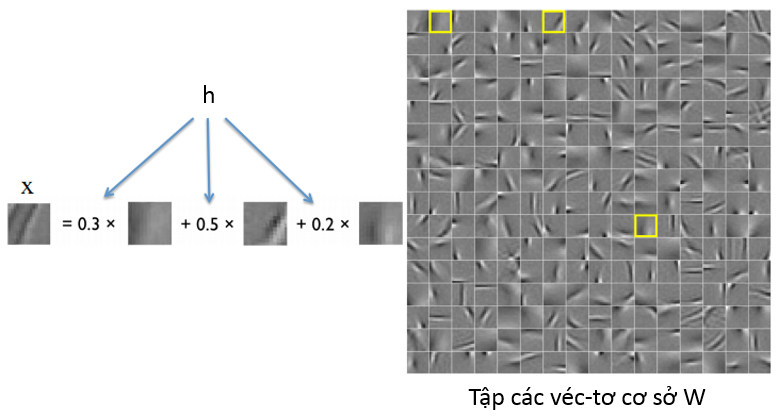
\includegraphics[width=\textwidth]{SparseCoding}
	\caption[Minh họa các đặc trưng học được của ``Sparse Coding'' khi huấn luyện trên ảnh tự nhiên]{Minh họa các đặc trưng (các véc-tơ cơ sở) học được của ``Sparse Coding'' khi huấn luyện trên ảnh tự nhiên \cite{zeiler2014thesis}. Các đặc trưng học được có dạng các cạnh ở các vị trí khác nhau và với các hướng khác nhau. Véc-tơ đầu vào $x$ có thể được tái tạo từ một số ít các đặc trưng trong tập các đặc trưng; nghĩa là, đa số các phần tử của véc-tơ đặc trưng (véc-tơ hệ số) $h$ bằng 0 (trong hình vẽ chỉ thể hiện các phần tử khác 0 của $h$).}
	\label{fig_SparseCoding}
\end{figure}
\section{"Variational Auto-Encoders"}
\subsection{Mô hình xác suất}
\subsection{"Variational Inferene"}
``Auto-Encoder'' đơn giản là một mạng nơ-ron truyền thẳng gồm có hai phần: 
\begin{itemize}
	\item Phần thứ nhất, được gọi là \emph{bộ mã hóa} (encoder), ánh xạ véc-tơ đầu vào $x \in \mathbb{R}^{D_x \times 1}$ sang véc-tơ biểu diễn ẩn $h \in \mathbb{R}^{D_h \times 1}$ theo công thức: 
	\begin{equation}
		h=f(W^{(e)}x + b^{(e)})
	\end{equation}
	Trong đó, $W^{(e)} \in \mathbb{R}^{D_h \times D_x}$ và $b^{(e)} \in \mathbb{R}^{D_h \times 1}$ là các tham số của bộ mã hóa. $f(\cdot)$ là một hàm kích hoạt nào đó; nói rõ hơn là, $f(\cdot)$ nhận đầu vào là một véc-tơ và trả về véc-tơ kết quả có cùng kích thước với véc-tơ đầu vào của $f(\cdot)$, trong đó mỗi phần tử của véc-tơ kết quả có được bằng cách áp dụng hàm kích hoạt (ví dụ, hàm sigmoid) lên phần tử tương ứng của véc-tơ đầu vào của $f(\cdot)$.
	\item Phần thứ hai, được gọi là \emph{bộ giải mã} (decoder), cố gắng tái tạo lại véc-tơ đầu vào $x$ ban đầu từ véc-tơ biễu diễn ẩn $h$:
	\begin{equation}
		\hat{x} = W^{(d)}h + b^{(d)}
	\end{equation}
	Trong đó, $\hat{x} \in \mathbb{R}^{D_x \times 1}$ là véc-tơ tái tạo, $W^{(d)} \in \mathbb{R}^{D_x \times D_h}$ và $b^{(d)} \in \mathbb{R}^{D_x \times 1}$ là các tham số của bộ giải mã.
\end{itemize}

Như vậy, từ véc-tơ đầu vào, ``Auto-Encoder'' ánh xạ sang véc-tơ biểu diễn ẩn; rồi từ véc-tơ biểu diễn ẩn này, ``Auto-Encoder'' cố gắng tái tạo lại véc-tơ đầu vào ban đầu (minh họa ở hình \ref{fig_AE}). Bằng cách này, ta hy vọng có thể thu được ở véc-tơ biểu diễn ẩn những thông tin có ích, giải thích dữ liệu quan sát được (véc-tơ đầu vào).

\begin{figure}
	\centering
	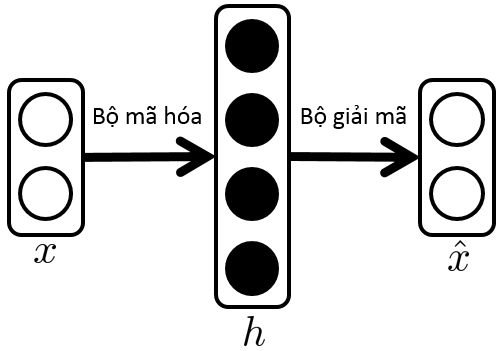
\includegraphics[scale=0.8]{AE}
	\caption{Minh họa ``Auto-Encoders''}
	\label{fig_AE}
\end{figure}
``Sparse Auto-Encoder'' (SAE) là một ``Auto-Encoder'' trong đó véc-tơ biểu diễn ẩn được ràng buộc thưa (nghĩa là, với một véc-tơ đầu vào, chỉ có một số nơ-ron ẩn kích hoạt). Một cách cụ thể, với một mẫu huấn luyện $x \in \mathbb{R}^{D_x}$, SAEs tối thiểu hóa hàm chi phí sau (tương tự như ``Sparse Coding'', để đơn giản về mặt ký hiệu, ở đây chúng tôi chỉ ghi hàm chi phí cho một mẫu huấn luyện; trong thực tế, mục tiêu là tối thiểu hóa chi phí trên toàn bộ tập huấn luyện và sự cập nhật các tham số có thể được tiến hành với một mẫu huấn luyện, hoặc với một số mẫu huấn luyện, hoặc với toàn bộ mẫu trong tập huấn luyện):
\begin{equation}
	C(W^{(e)}, b^{(e)}, W^{(d)}, b^{(d)}) = ||x - \hat{x}||_2^2 + \lambda s(h)
	\label{eq_SAE}
\end{equation}
Trong đó, $\hat{x}$ là véc-tơ tái tạo (với $\hat{x} = W^{(d)}h + b^{(d)}$ và $h = f(W^{(e)}x + b^{(e)})$); $s(\cdot)$ là một hàm nào đó mà làm cho véc-tơ biểu diễn ẩn $h$ thưa (ví dụ, $s(\cdot)$ có thể là chuẩn L1 như ở ``Sparse Coding''); và $\lambda$ là siêu tham số điều khiển ``sự thỏa hiệp'' giữa độ lỗi tái tạo và độ thưa.

Như vậy, ta thấy rằng, mục tiêu của SAEs giống với ``Sparse Coding'', đó là tìm ra véc-tơ biểu diễn đặc trưng (véc-tơ biểu diễn ẩn) thỏa hai tính chất:
\begin{itemize}
	\item Có thể tái tạo tốt véc-tơ đầu vào.
	\item Thưa.
\end{itemize}

Tuy nhiên, điểm khác biệt giữa chúng là (minh họa ở hình \ref{fig_SCvsSAE}): SAEs có bộ mã hóa \emph{cụ thể, có tham số} (nghĩa là, có hàm cụ thể ánh xạ từ véc-tơ đầu vào sang véc-tơ đặc trưng); trong khi đó, bộ mã hóa của ``Sparse Coding'' \emph{không cụ thể, không có tham số} (nghĩa là, không có hàm cụ thể ánh xạ từ véc-tơ đầu vào sang véc-tơ đặc trưng). Điểm khác biệt này giúp cho SAEs có một số lợi thế so với ``Sparse Coding'':
\begin{itemize}
	\item Việc huấn luyện SAEs có thể được thực hiện hiệu quả hơn ``Sparse Coding'' thông qua thuật toán lan truyền ngược.
	\item Sau khi huấn luyện, với một véc-tơ đầu vào mới, SAEs có thể tính ra được véc-tơ đặc trưng rất nhanh bằng cách lan truyền tiến qua bộ mã hóa; trong khi đó, ``Sparse Coding'' vẫn phải tiến hành quá trình tối ưu hóa.
\end{itemize}

\begin{figure}
	\centering
	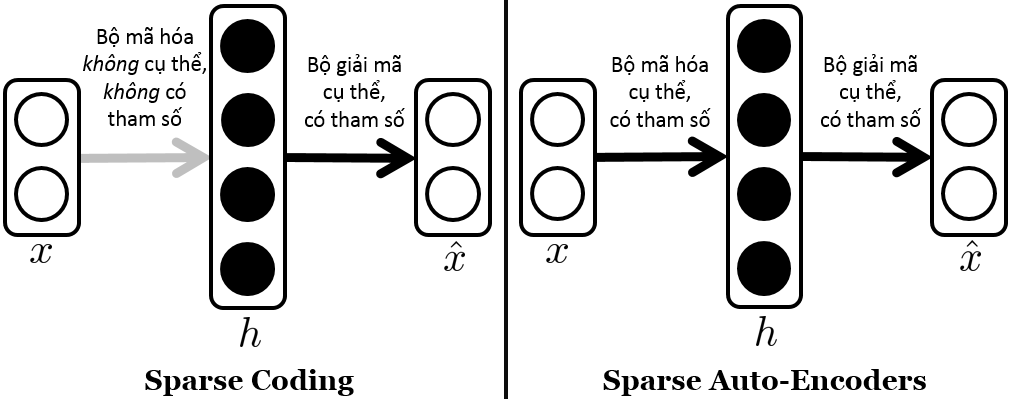
\includegraphics[width=\textwidth]{SCvsSAE}
	\caption[So sánh giữa ``Sparse Coding'' và SAEs]{So sánh giữa ``Sparse Coding'' và SAEs. SAEs có bộ mã hóa \emph{cụ thể, có tham số} ($h = f(W^{(e)}x + b^{(e)})$); trong khi đó, bộ mã hóa của ``Sparse Coding'' \emph{không cụ thể, không có tham số}.}
	\label{fig_SCvsSAE}
\end{figure}

\subsection{"Kullback-Leiber Devergence"}
``Softmax Regression'' là mô hình phân $K$ lớp. Trong ngữ cảnh của bài toán học đặc trưng, ``Softmax Regression'' thường được dùng để đánh giá các đặc trưng học được (bởi mô hình này đơn giản, không có nhiều siêu tham số).

Cho tập huấn luyện $\{(x^{(1)}, y^{(1)}), \ldots, (x^{(N)}, y^{(N)})\}$. Để tìm ra được các tham số $W$ và $b$ của hàm dự đoán của ``Softmax Regression'' ở công thức (\ref{eq_SoftmaxHypotheses}), ta sẽ dùng phương pháp ``maximum likelihood''. Giả sử các mẫu dữ liệu trong tập huấn luyện được phát sinh một cách độc lập với nhau, ta có hàm ``likelihood'':
\begin{equation}
\begin{split}
	L(W, b) &= p(Y|X)\\
			&= \prod_{i=1}^{N} p(y^{(i)}|x^{(i)})\\
			&= \prod_{i=1}^{N} \prod_{j=1}^K \left(\frac{\exp(W_j^Tx + b_j)}{\sum_{k=1}^{K}\exp(W_k^Tx + b_k)}\right)^{1\{y^{(i)}=j\}}\\
\end{split}
\end{equation}
Trong đó:
\begin{itemize}
	\item $X = \{x^{(1)}, \ldots, x^{(N)}\}$ và $Y = \{y^{(1)}, \ldots, y^{(N)}\}$.
	\item Hàm ${1\{y^{(i)}=j\}}$ sẽ trả về $1$ nếu $y^{(i)}=j$ và trả về $0$ nếu ngược lại.
\end{itemize}
Ta tìm $W$ và $b$ sao cho hàm ``likelihood'' $L(W, b)$ đạt cực đại. Cực đại $L(W, b)$ tương đương với cực tiểu $-\log L(W, b)$ (hàm này được gọi là hàm ``negative log-likelihood'').

Như vậy, ta sẽ tìm các tham số $W$ và $b$ của hàm dự đoán của ``Softmax Regression'' sao cho hàm chi phí sau đạt cực tiểu:
\begin{equation}
\begin{split}
	C(W, b) &= -\log L(W, b)\\
			&= -\sum_{i=1}^{N}\sum_{j=1}^{K} 1\{y^{(i)}=j\} \log \frac{\exp(W_j^Tx + b_j)}{\sum_{k=1}^{K}\exp(W_k^Tx + b_k)}
\end{split}
\end{equation}
Để cực tiểu hóa hàm này, ta có thể sử dụng thuật toán ``Gradient Descent'' (sẽ được trình bày ở dưới).



\section{"Loglikelihood function"}

Thuật toán ``Batch Gradient Descent'' (BGD) dùng để cực tiểu hóa hàm chi phí $C(W)$ \emph{trên toàn bộ tập huấn luyện} theo tham số $W$ (ví dụ, $C(W)$ có thể là hàm chi phí trên toàn bộ tập huấn luyện của ``Auto-Encoders'' hay của ``Softmax Regression''). Một cách cụ thể, xét hàm chi phí trên toàn bộ tập huấn luyện của một mô hình học nào đó (ví dụ, ``Auto-Encoders'' hay ``Softmax Regression''):
\begin{equation}
	C(W) = \frac{1}{N} \sum_{i=1}^N C^{(i)}(W)
	\label{eq_CostFunct}
\end{equation}
Trong đó:
\begin{itemize}
	\item $W$ là các tham số của mô hình học.
	\item $C^{(i)}(W)$ là chi phí của mẫu huấn luyện thứ $i$ trong tập huấn luyện.
	\item $N$ là tổng số mẫu huấn luyện.
\end{itemize}
Mục tiêu của ta là tìm $W$ để $C(W)$ đạt cực tiểu.

Ý tưởng của BGD là đầu tiên khởi tạo ngẫu nhiên $W$, rồi nhìn vùng cục bộ xung quanh $W$ và đi (cập nhật $W$) theo hướng mà làm cho $C(W)$ giảm nhiều nhất; tại $W$ mới, ta lại lặp lại qui trình này: nhìn vùng cục bộ xung quanh $W$ và đi theo hướng mà làm cho $C(W)$ giảm nhiều nhất; cứ thế..., ta lặp cho đến khi hội tụ. Hình \ref{fig_BGD} minh họa cho quá trình chạy này của BGD với trường hợp đơn giản là $W$ chỉ gồm có 2 thành phần là $W_0$ và $W_1$.
\begin{figure}
	\centering
	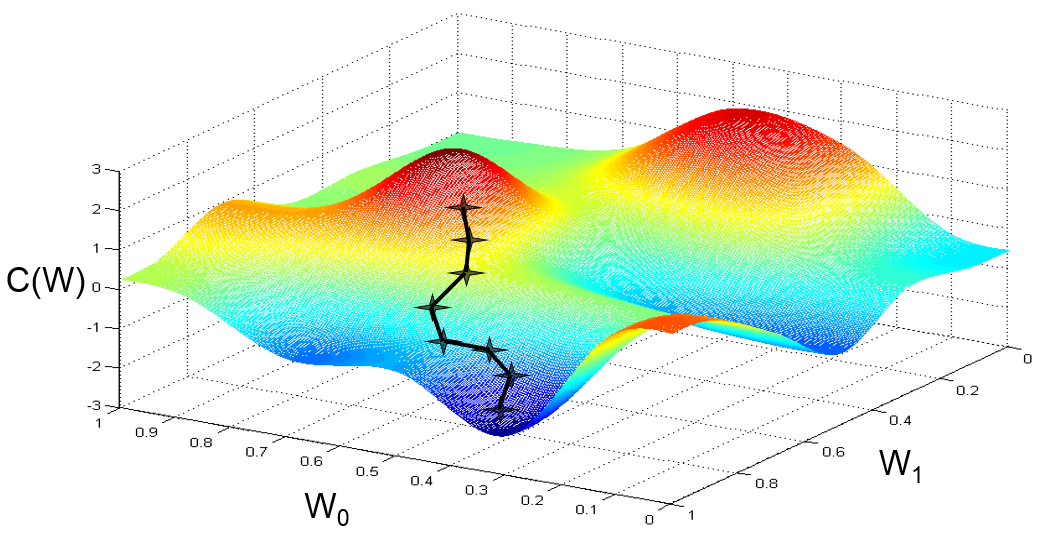
\includegraphics[width=\textwidth]{BGD}
	\caption[Minh họa quá trình chạy của thuật toán BGD]{Minh họa quá trình chạy của thuật toán BGD (hình vẽ được điều chỉnh từ hình vẽ lấy từ slide bài giảng của GS. Andrew Ng trong lớp máy học trực tuyến ở trang \url{coursera.org}).}
	\label{fig_BGD}
\end{figure}

Cụ thể, ở mỗi vòng lặp, ta sẽ cập nhật $W$ theo công thức:
\begin{equation}
	W = W + \eta \hat{v}
\end{equation}
Trong đó:
\begin{itemize}
	\item $\hat{v}$ là véc-tơ đơn vị có cùng kích thước với $W$ cho biết hướng đi (hướng cập nhật $W $) mà sẽ làm cho $C(W)$ giảm nhiều nhất xét trong vùng cục bộ xung quanh $W$ hiện tại.
	\item $\eta$ là hằng số dương điều khiển độ dài của một bước đi.
\end{itemize}
Ta nên đi theo hướng $\hat{v}$ nào để làm cho $C(W)$ giảm nhiều nhất xét trong vùng cục bộ xung quanh $W$ hiện tại? Xét hiệu sau:
\begin{equation}
	\Delta C = C(W + \eta \hat{v}) - C(W)
	\label{eq_DeltaC}
\end{equation}
Ta cần tìm $\hat{v}$ để làm cho $\Delta C$ có giá trị âm nhỏ nhất. BGD xấp xỉ $C(W + \eta \hat{v})$ bằng cách sử dụng khai triển Taylor \emph{đến số hạng ứng với đạo hàm bậc nhất} (để ý $W + \eta \hat{v}$ là điểm lân cận xung quanh $W$):
\begin{equation}
	C(W + \eta \hat{v}) \approx C(W) + \eta \nabla C(W)^T \hat{v}
	\label{eq_TalorExpansion}
\end{equation}
với $\nabla C(W)$ là véc-tơ chứa các đạo hàm riêng của $C$ theo $W$ (ở đây, khi nói đến véc-tơ, ta ngầm hiểu là véc-tơ cột). Thế công thức (\ref{eq_TalorExpansion}) vào công thức (\ref{eq_DeltaC}) ta được:
\begin{equation}
\begin{split}
	\Delta C &= \eta \nabla C(W)^T \hat{v}\\
			 &= \eta \|\nabla C(W)\|\|\hat{v}\|\cos \left(\nabla C(W);\hat{v}\right)\\
			 &= \eta \|\nabla C(W)\|\cos \left(\nabla C(W);\hat{v}\right)\\
			 &\geq - \eta \|\nabla C(W)\|
\end{split}
\end{equation}
Ta thấy $\Delta C$ sẽ có giá trị âm nhỏ nhất khi $\cos$ của góc tạo bởi hai véc-tơ $\nabla C(W)$ và $\hat{v}$ có giá trị bằng $-1$; nghĩa là, $\hat{v}$ sẽ có chiều ngược với chiều của $C(W)$. Và vì $\hat{v}$ là véc-tơ đơn vị nên cuối cùng ta có:
\begin{equation}
	\hat{v} = -\frac{\nabla C(W)}{\|\nabla C(W)\|}
\end{equation}
Như vậy, ta có công thức cập nhật tham số ở mỗi vòng lặp của BGD như sau:
\begin{equation}
	W = W -\eta \frac{\nabla C(W)}{\|\nabla C(W)\|}
	\label{eq_UpdateW_FixedStep}
\end{equation}

Với công thức cập nhật tham số trên, ở mỗi vòng lặp, BGD sẽ luôn đi một bước có độ dài cố định là $\eta$. Tuy nhiên, ta thấy rằng khi $\|\nabla C(W)\|$ lớn (độ dốc lớn), ta muốn đi một bước dài; và khi $\|\nabla C(W)\|$ nhỏ (độ dốc nhỏ, nhiều khả năng gần cực trị), ta muốn đi một bước ngắn. Nghĩa là, thay vì dùng độ dài bước đi $\eta$ cố định, ta muốn dùng $\eta$ thay đổi và tỉ lệ thuận với $\|\nabla C(W)\|$:
\begin{equation}
	\eta = \alpha \|\nabla C(W)\|
	\label{eq_VariableStep}
\end{equation}
với $\alpha$ là hằng số dương cho biết mức độ tỉ lệ thuận giữa $\|\nabla C(W)\|$ và $\eta$; $\alpha$ được gọi là hệ số học (learning rate). Thế (\ref{eq_VariableStep}) vào (\ref{eq_UpdateW_FixedStep}) ta được công thức cập nhật tham số của BGD:
\begin{equation}
	W = W - \alpha \nabla C(W)
	\label{eq_UpdateW_VariabeStep}
\end{equation}
Nếu $\alpha$ lớn thì ta sẽ đi được một bước dài nhưng có nguy cơ ra khỏi vùng xấp xỉ cục bộ của khai triển Taylor (nghĩa là không đảm bảo sau khi cập nhật $W$ sẽ làm cho giá trị của hàm chi phí $C$ giảm). Nếu $\alpha$ nhỏ thì sẽ đảm bảo nằm trong vùng xấp xỉ cục bộ của khai triển Taylor nhưng thời gian học sẽ rất lâu (vì mỗi lần cập nhật chỉ đi được một bước ngắn). Do đó, cần chọn giá trị $\alpha$ trung dung.

%\begin{leftbar}
%Từng bước của thuật toán BGD như sau:
%	\begin{enumerate}
%		\item Khởi tạo ngẫu nhiên cho $W$.
%		\item Lặp cho đến khi thỏa điều kiện dừng:
%		\[
%			W = W - \alpha \nabla C(W)
%		\]
%		($\alpha>0$ là hệ số học)
%	\end{enumerate}
%\end{leftbar}

Tổng thể thuật toán BGD được trình bày ở thuật toán \ref{alg_BGD}. Cách xác định điều kiện dừng của thuật toán sẽ được trình bày ở mục \ref{sec_early_stopping}.
\begin{algorithm}
	\newalgname{Thuật toán}
	\caption{Batch Gradient Descent (BGD)}
	\label{alg_BGD}
	\begin{algorithmic}[1]
		\renewcommand{\algorithmicrequire}{\textbf{Đầu vào:}}
		\renewcommand{\algorithmicensure}{\textbf{Đầu ra:}}
		\algnewcommand\algorithmicoperation{\textbf{Thao tác:}}
		\algnewcommand\Operation{\item[\algorithmicoperation]}
		
		\Require Tập huấn luyện, hệ số học $\alpha>0$
		\Ensure Bộ tham số $W$ của mô hình học để cho hàm chi phí $C(W)$ đạt cực tiểu
		
		\Operation
		\State Khởi tạo ngẫu nhiên cho $W$
		\While{chưa thỏa điều kiện dừng}
			\State $W = W - \alpha \nabla C(W)$ \%\% $C$ là hàm chi phí trên toàn bộ tập huấn luyện
		\EndWhile
	\end{algorithmic}
\end{algorithm}

Thuật toán ``Stochastic Gradient Descent'' (SGD) là cải tiến của ``Batch Gradient Descent'' (BGD) để tăng tốc quá trình tối ưu hóa khi phải làm việc với tập dữ liệu lớn. Một cách cụ thể, xét công thức cập nhật tham số (\ref{eq_UpdateW_VariabeStep}) của BGD, ta thấy để đi một bước (thực hiện một lần cập nhật $W$), ta cần phải tính véc-tơ đạo hàm riêng $\nabla C(W)$. Từ công thức (\ref{eq_CostFunct}) của hàm chi phí $C(W)$ ta có:
\begin{equation}
	\nabla C(W) = \frac{1}{N} \sum_{i=1}^N \nabla C^{(i)}(W)
\end{equation}
Nghĩa là với BGD, để đi được một bước, ta cần phải duyệt hết toàn bộ tập huấn luyện để tính các véc-tơ đạo hàm riêng $\nabla C^{(i)}(W)$ của hàm chi phí của mỗi mẫu huấn luyện, rồi sau đó lấy trung bình các véc-tơ đạo hàm riêng này để ra được $\nabla C(W)$. Khi mà tập huấn luyện lớn, quá trình này sẽ tốn thời gian và làm cho BGD chạy rất chậm.

SGD khắc phục nhược điểm trên của BGD bằng cách: thay vì phải duyệt tất cả các mẫu trong tập huấn luyện và tính véc-tơ đạo hàm riêng trung bình rồi mới đi được một bước như ở BGD, SGD chỉ duyệt qua \emph{một số mẫu} trong tập huấn luyện, tính véc-tơ đạo hàm riêng trung bình \emph{trên tập con này}, rồi đã đi ngay một bước. Ví dụ, với tập huấn luyện có $1000$ mẫu, BGD sẽ duyệt qua hết $1000$ mẫu này rồi mới đi được một bước; trong khi đó, với $10$ mẫu đầu tiên, SGD đi được một bước, với $10$ mẫu kế tiếp, SGD đi được một bước nữa... (ở đây, giả sử số lượng mẫu mà SGD cần duyệt qua để đi được một bước là $10$). Như vậy, với một lần quét qua toàn bộ tập huấn luyện, BGD chỉ đi được $1$ bước, trong khi đó SGD đi được tới $100$ bước. Nguyên $1000$ mẫu được gọi là một ``batch'', còn tập gồm $10$ mẫu để SGD đi được một bước gọi là một ``mini-batch''; ở đây, ta nói kích thước của ``mini-batch'' bằng $10$. Một lần duyệt qua toàn bộ tập huấn luyện được gọi là một ``epoch''; như vậy, SGD sẽ thực hiện nhiều ``epoch'', trong mỗi ``epoch'' lại thực hiện nhiều lần cập nhật tham số ứng với các ``mini-batch''.

Tại sao SGD hoạt động? Ta thấy hướng đi của BGD được tính bằng cách lấy trung bình trên \emph{toàn bộ tập huấn luyện} các véc-tơ đạo hàm riêng $\nabla C^{(i)}(W)$, còn hướng đi của SGD được tính bằng cách lấy trung bình trên \emph{một tập con (một ``mini-batch'') của tập huấn luyện} các véc-tơ đạo hàm riêng $\nabla C^{(i)}(W)$. Như vậy, tuy hướng đi của SGD không chính xác hoàn toàn với hướng đi của BGD nhưng nó sẽ giao động xung quanh hướng đi của BGD; hay nói một cách khác, hướng đi của SGD xấp xỉ hướng đi của BGD. Nếu ta chọn kích thước của ``mini-batch'' nhỏ (tối thiểu là bằng $1$) thì SGD sẽ chạy nhanh nhưng độ ``nhiễu loạn'' (độ giao động xung quanh hướng đi của BGD) sẽ tăng; còn nếu ta chọn kích thước của ``mini-batch'' lớn (tối đa là bằng số lượng mẫu của tập huấn luyện, lúc này SGD trở thành BGD) thì độ ``nhiễu loạn'' sẽ giảm nhưng SGD sẽ chạy chậm. Do đó, cần chọn kích thước ``mini-batch'' có giá trị trung dung. Lưu ý là tính ``nhiễu loạn'' của SGD cũng sẽ thể có lợi khi hàm chi phí có ``bề mặt'' phức tạp (ví dụ như hàm chi phí của mạng nơ-ron); chẳng hạn, tính ``nhiễu loạn'' có thể giúp SGD ``nhảy'' ra khỏi những vùng cực trị cục bộ, hay không bị mắc kẹt ở những vùng ``đồng bằng''. Ngoài ra, khi chọn kích thước của ``mini-batch'' $>1$, ta sẽ có thể tận dụng được sức mạnh tính toán song song.

%\begin{leftbar}
%Từng bước của thuật toán SGD như sau:
%\begin{enumerate}
%	\item Khởi tạo ngẫu nhiên cho $W$.
%	\item Lặp cho đến khi thỏa điều kiện dừng:
%	\begin{itemize}
%		\item Xáo trộn ngẫu nhiên thứ tự của các mẫu trong tập huấn luyện (thường sẽ giúp SGD hội tụ nhanh hơn).
%		\item Với $b=1,2,\ldots,\frac{N}{B}$ ($N$ là số lượng mẫu trong tập huấn luyện, $B$ là kích thước của ``mini-batch''), cập nhật $W$ theo công thức:
%		\[W = W - \alpha \frac{1}{B} \sum_{i=(b-1)B+1}^{bB} \nabla C^{(i)}(W)\]
%		($\alpha > 0$ là hệ số học)
%	\end{itemize}
%\end{enumerate}
%\end{leftbar}

Tổng thể thuật toán SGD được trình bày ở thuật toán \ref{alg_SGD}. Cách xác định điều kiện dừng của thuật toán sẽ được trình bày ở mục \ref{sec_early_stopping}.
\begin{algorithm}
	\newalgname{Thuật toán}
	\caption{Stochastic Gradient Descent (SGD)}
	\label{alg_SGD}
	\begin{algorithmic}[1]
		\renewcommand{\algorithmicrequire}{\textbf{Đầu vào:}}
		\renewcommand{\algorithmicensure}{\textbf{Đầu ra:}}
		\algnewcommand\algorithmicoperation{\textbf{Thao tác:}}
		\algnewcommand\Operation{\item[\algorithmicoperation]}
		
		\Require Tập huấn luyện gồm $N$ mẫu, hệ số học $\alpha>0$, kích thước ``mini-batch'' B
		\Ensure Bộ tham số $W$ của mô hình học để cho hàm chi phí $C(W)$ đạt cực tiểu
		
		\Operation
		\State Khởi tạo ngẫu nhiên cho $W$
		\While{chưa thỏa điều kiện dừng} \%\% Với mỗi ``epoch''
			\State \parbox[t]{\dimexpr\linewidth-\algorithmicindent}{Xáo trộn ngẫu nhiên thứ tự của các mẫu trong tập huấn luyện (thường sẽ giúp SGD hội tụ nhanh hơn)\strut}
			\For{b = 1 : N/B} \%\% Với mỗi ``mini-batch''
				\State $W = W - \alpha \frac{1}{B} \sum_{i=(b-1)B+1}^{bB} \nabla C^{(i)}(W)$ 
			\EndFor
		\EndWhile
	\end{algorithmic}
\end{algorithm}


``Dừng sớm'' (early stopping) là một cách ``miễn phí'' để quyết định số vòng lặp của SGD (hay BGD). Sở dĩ nói ``miễn phí'' là vì để chọn một siêu tham số, thông thường ta cần phải tiến hành huấn luyện nhiều lần với các giá trị khác nhau của siêu tham số này, và chọn ra giá trị mà cho kết quả tốt nhất trên tập ``validation'' (tập ngoài tập huấn luyện); ở đây, với chiến lược ``dừng sớm'', số lượng vòng lặp sẽ được xác định ngay trong quá trình huấn luyện (nghĩa là, chỉ tốn một lần huấn luyện). Ngoài ra, chiến lược ``dừng sớm'' cũng giúp chống vấn đề quá khớp (overfitting).

Ý tưởng của chiến lược ``dừng sớm'' đơn giản là trong khi thực hiện các vòng lặp của quá trình tối ưu hóa với SGD (hay BGD), ta sẽ theo dõi ``độ lỗi'' trên tập ``validation'' (ở đây, ``độ lỗi'' được định nghĩa tùy theo ngữ cảnh; ví dụ, nếu dùng SGD để cực tiểu hóa hàm chi phí của ``Softmax Regression'' thì ``độ lỗi'' có thể là tỉ lệ phân lớp sai, còn nếu dùng SGD để cực tiểu hóa hàm chi phí của SAEs thì ``độ lỗi'' có thể là giá trị của hàm chi phí). Khi SGD (hay BGD) càng thực hiện nhiều vòng lặp thì nhìn chung ``độ lỗi'' trên tập huấn luyện sẽ càng giảm xuống, còn ``độ lỗi'' trên tập ``validation'' (ngoài tập huấn luyện) ban đầu sẽ giảm xuống nhưng đến một lúc nào đó sẽ tăng lên, báo hiệu bắt đầu xảy ra sự quá khớp. Do đó, trong quá trình tối ưu hóa với SGD (hay BGD), nếu thấy ``độ lỗi'' trên tập ``validation'' tăng lên thì ta sẽ dừng quá trình tối ưu hóa. Ý tưởng này của chiến lược ``dừng sớm'' được minh họa ở hình \ref{fig_EarlyStopping}.

\begin{figure}
	\centering
	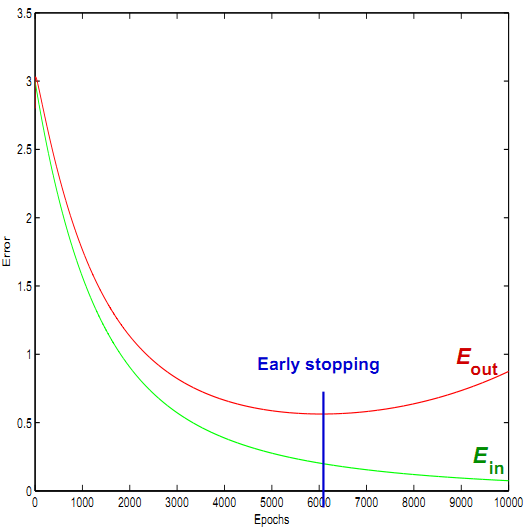
\includegraphics[scale=0.9]{EarlyStopping}
	\caption[Minh họa chiến lược ``dừng sớm'']{Minh họa chiến lược ``dừng sớm'' (early stopping). $E_{in}$ là độ lỗi trên tập huấn luyện, còn $E_{out}$ là độ lỗi trên tập ``validation'' (ngoài tập huấn luyện).}
	\label{fig_EarlyStopping}
\end{figure}

Trong thực tế cài đặt, khi thấy ``độ lỗi'' trên tập ``validation'' tăng lên, ta không nên dừng ngay quá trình tối ưu hóa mà nên thực hiện thêm một số vòng lặp nữa rồi mới quyết định dừng hay không (bởi vì có thể ``độ lỗi'' trên tập ``validation'' chỉ tăng lên một tí rồi sau đó lại giảm xuống). 


